
%(BEGIN_QUESTION)
% Copyright 2011, Tony R. Kuphaldt, released under the Creative Commons Attribution License (v 1.0)
% This means you may do almost anything with this work of mine, so long as you give me proper credit

This control system measures and regulates the amount of differential pressure across a gas compressor, by opening a {\it recirculation} valve to let high-pressure discharge gas go back to the low-pressure ``suction'' of the compressor.  This control system needs to be very fast-acting, and currently it is anything but that, as revealed by the open-loop trend shown in the upper-right of this illustration:

$$\includegraphics[width=15.5cm]{i02324x01.eps}$$

After inspecting the trend graph, you decide to walk out of the control room and over to the compressor where you can observe the valve stem move.  You then call the control room operator on your two-way radio and ask him to move the control valve (in manual) back to its starting position.  What you see is a very quick, crisp motion from the control valve: no hesitation and no overshoot.  The PDT trend still takes several seconds to stabilize, though.

\vskip 10pt

Identify what type of problem you think you are dealing with here, as the compressor's differential pressure should {\it not} take several seconds to stabilize following a sudden move by the recirculation valve.  Also suggest a next diagnostic test or measurement to take, explaining how the result(s) of that test helps further identify the location and/or nature of the fault.

\vskip 20pt \vbox{\hrule \hbox{\strut \vrule{} {\bf Suggestions for Socratic discussion} \vrule} \hrule}

\begin{itemize}
\item{} Explain why the first test of observing valve motion was a very good decision.  What specifically did the result of that test tell you about the nature and/or location of the fault?
\end{itemize}

\underbar{file i02324}
%(END_QUESTION)





%(BEGIN_ANSWER)

The problem is clearly on the measurement side of this control loop: the controller (for whatever reason) is not ``seeing'' the change in DP across the compressor as quickly as it should.  I will leave it to you to determine how to isolate the problem.  

\vskip 10pt

Hint: {\it use your multimeter!}

%(END_ANSWER)





%(BEGIN_NOTES)

Here is a list of potential problems:

\begin{itemize}
\item{} Transmitter not sensing pressure quickly, due to partial plugs in impulse line(s) or partially closed block valve(s)
\item{} Transmitter has filtering enabled
\item{} Controller input has filtering enabled
\item{} Valve plug uncoupled from stem inside the valve body
\end{itemize}

A quick voltage or current measurement on the transmitter circuit during another step-change in valve position will tell you whether or not the transmitter is sending the proper (quick-changing) signal to the controller.  If so, the controller is at fault (input filtering?).  If not, the transmitter or its impulse tube connections is/are at fault.

\vfil \eject

$$\includegraphics[width=15.5cm]{i02324x02.eps}$$






\filbreak \vskip 20pt \vbox{\hrule \hbox{\strut \vrule{} {\bf Virtual Troubleshooting} \vrule} \hrule}

\noindent
{\bf Predicting the effect of a given fault:} present each of the following faults to the students, one at a time, having them comment on all the effects each fault would produce.

\begin{itemize}
\item{} I/P nozzle plugs
\item{} Volume booster restrictor plugs
\item{} Controller output cable fails open
\item{} Controller output cable fails shorted
\item{} Transmitter cable fails open
\item{} Transmitter cable fails shorted
\item{} Instrument air supply fails
\item{} Transmitter block valve shut
\item{} Transmitter equalizing valve open
\item{} PDIC configured for reverse action instead of direct action
\end{itemize}


\vskip 10pt


\noindent
{\bf Identifying possible/impossible faults:} present symptoms to the students and then have them determine whether or not a series of suggested faults could account for all the symptoms, explaining {\it why} or {\it why not} for each proposed fault:

\begin{itemize}
\item{} Symptom: {\it }
\item{} 
\item{} 
\item{} 
\end{itemize}


\vskip 10pt


\noindent
{\bf Determining the utility of given diagnostic tests:} present symptoms to the students and then propose the following diagnostic tests one by one.  Students rate the value of each test, determining whether or not it would give useful information (i.e. tell us something we don't already know).  Students determine what different results for each test would indicate about the fault, if anything:

\begin{itemize}
\item{} Symptom: {\it }
\item{}  -- {\bf Yes/No}
\item{}  -- {\bf Yes/No}
\end{itemize}


\vskip 10pt


\noindent
{\bf Diagnosing a fault based on given symptoms:} imagine the ??? fails ??? in this system (don't reveal the fault to students!).  Present the operator's observation(s) to the students, have them consider possible faults and diagnostic strategies, and then tell them the results of tests they propose based on the following symptoms, until they have properly identified the nature and location of the fault:

\begin{itemize}
\item{} {\it }
\item{} 
\item{} 
\end{itemize}





%INDEX% Basics, control loop troubleshooting: determining location of signal filtering
%INDEX% Process: compressor differential pressure control
%INDEX% Process: compressor surge control

%(END_NOTES)

